\section{CPU usage}
	The anontunnels create a Tribler session, run multiple cryptographic functions and are relaying and downloading data. Each of these operations require CPU utilization. As this application will be merged with the other bachelor group (TSAP), we have to make sure that the CPU still has computational power available for the video playback.
	
	To ensure this, we have ran some CPU usage tests under three activities:
	
	\begin{enumerate}
		\item Measure CPU usage when idle. The application is in an idle state when it's searching and building circuits and not downloading/relaying data.
		\item Measure CPU usage when downloading. The application will download a 50M test file.
		\item Measure CPU usage when relaying. This means going from idle to creating circuits to pass on data that is downloaded by another node in the network.
	\end{enumerate}
	
	\subsection{CPU usage when idle}
		We first measured the CPU usage when the application is idle. We measured the speed and in figure 4.1, an overview of the CPU usage is given. The first characterize we can see is the peak after about 20 seconds. This is the startup of a Tribler session and as we can see, it is quite CPU heavy. When starting up Tribler, we initialize the database, start Dispersy and load the proxy community. Starting up Tribler does not take long (it takes about one or two seconds) and after the startup, the average CPU usage is about 18\%. The usage is a bit volatile which can be due to the processing of incoming and outgoing packets.
	
		\begin{figure*}[!t]
			\centering
			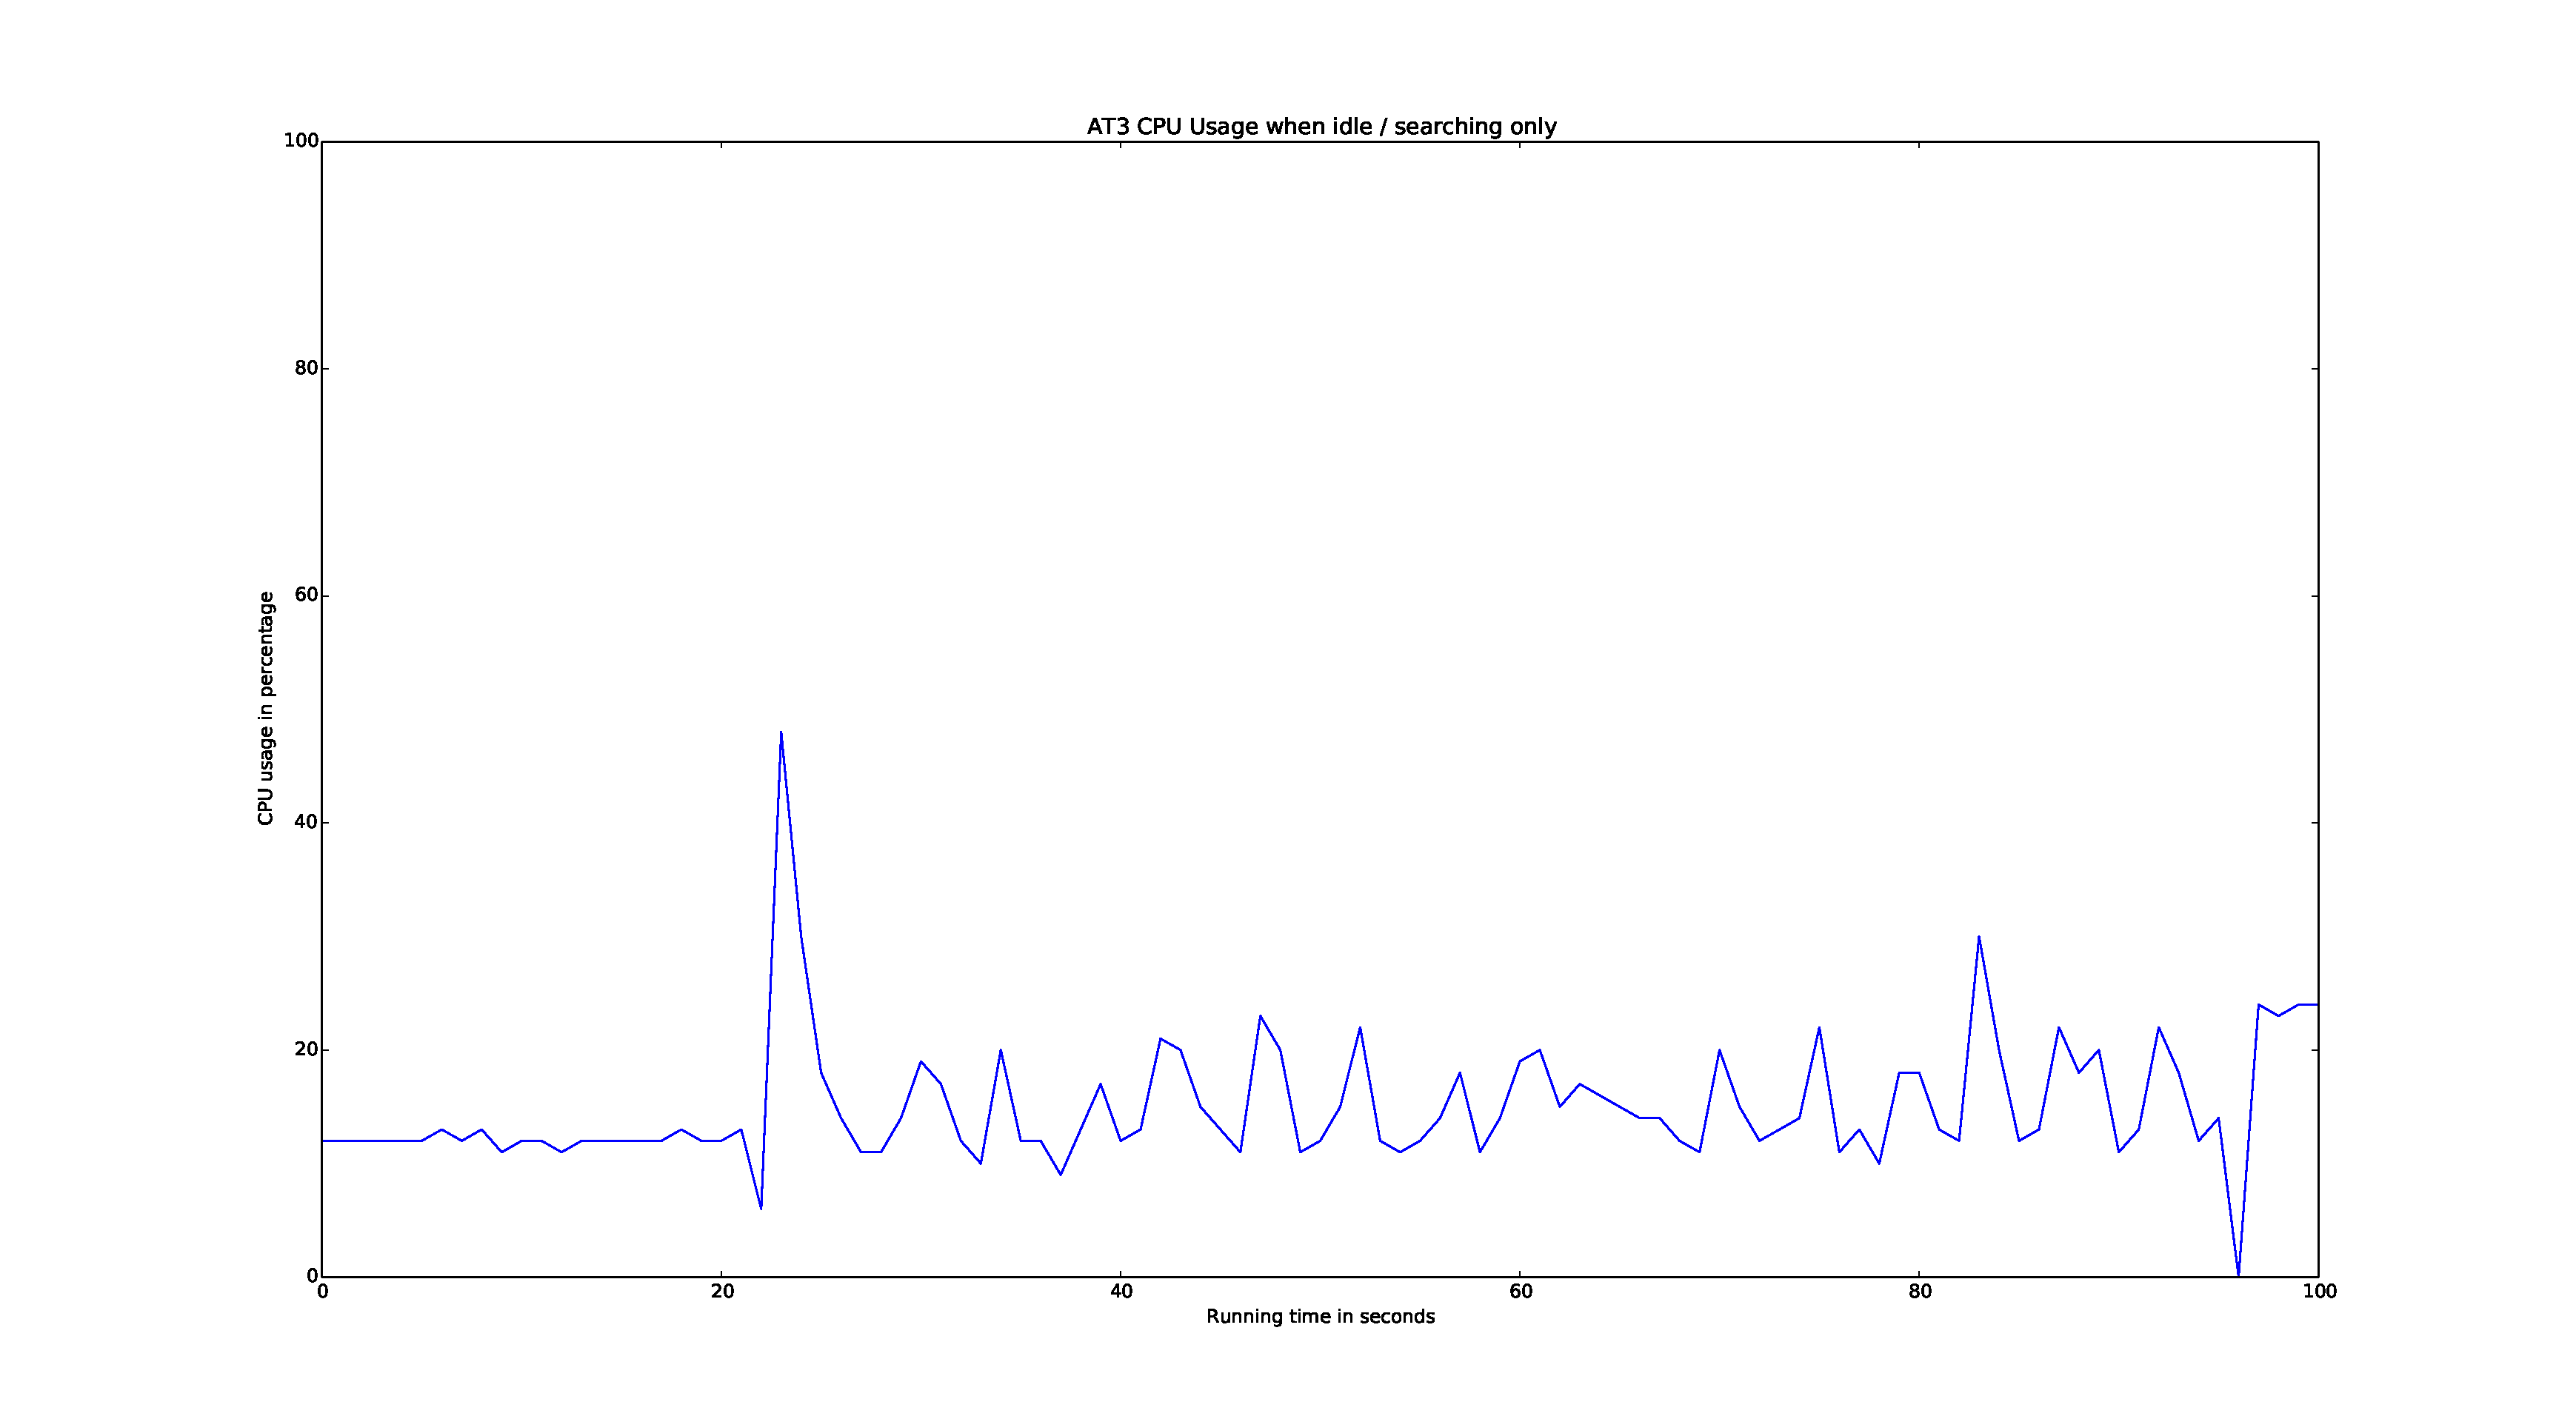
\includegraphics[width=0.8\textwidth]{graphics/cpu_idle.pdf}
			\caption{The CPU usage of AT3 when in the idle state.}
			\label{fig:cpu_idle_graph}
		\end{figure*}
		
		\subsection{CPU usage when downloading}
			Another important measurement is the CPU usage when downloading. We first download a 50M test file over one hop with one circuit. After that, we performed the same download but now with one circuit with a three hop length. This is of particular interest because we would like to stream a video. This mean that we simultaneously download and playback the video. We do not want high CPU usage when downloading because the video playback also needs CPU power. In figure 4.2 and figure 4.3 we present the graphs of these runs.
			
			\begin{figure*}[!t]
				\centering
				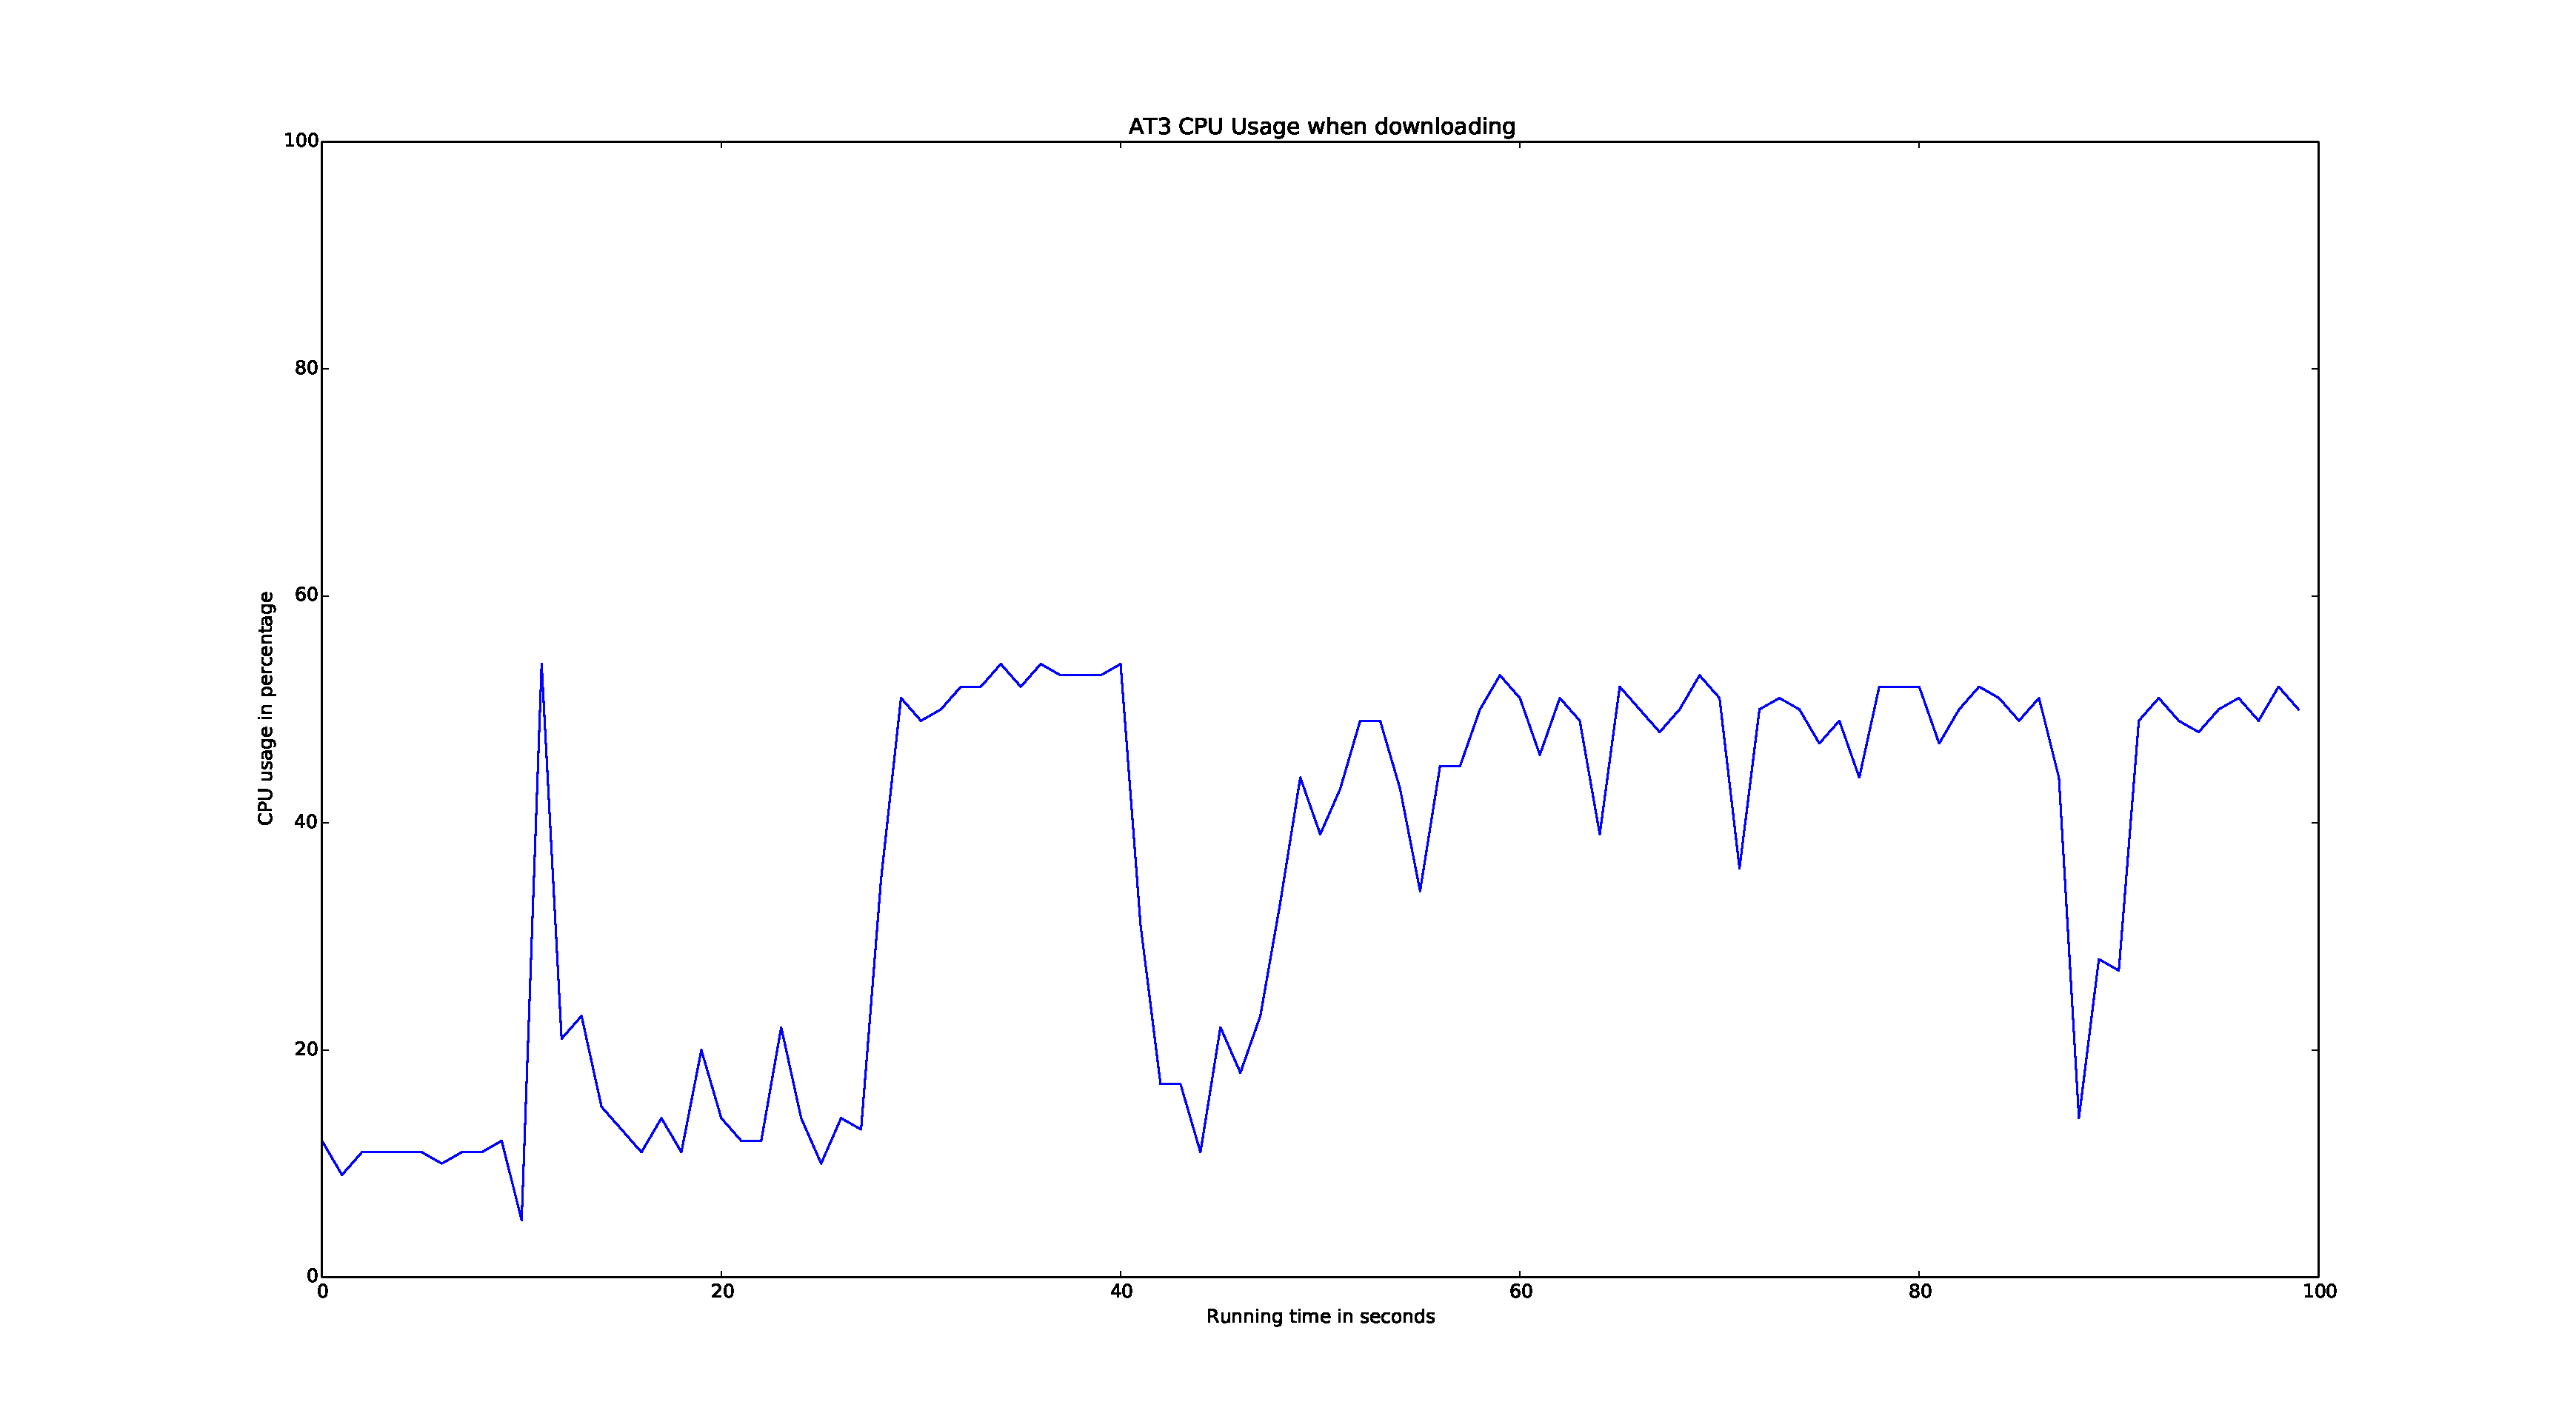
\includegraphics[width=0.8\textwidth]{graphics/cpu_downloading.pdf}
				\caption{The CPU usage of AT3 when downloading over one hop and with one circuit.}
				\label{fig:cpu_idle_graph}
			\end{figure*}